\chapter{Plastics and Synthetic Materials}\label{ch:g8:plastics}

Count the \omterm{def:g8:plastics:plastic}{plastic} objects you touch in one morning: a toothbrush, a
bottle, a raincoat, a phone case, the seat of a bus, the bag of the
shopping. Hardly any of them existed a hundred and twenty years ago, and
none of them grew on a tree or was dug out of the ground. \omterm{def:g8:plastics:plastic}{Plastics} are
materials invented by chemists --- light, cheap, waterproof, shaped into
anything --- and that very success has become a problem.

\begin{recall}
\omterm{def:g5:raw-materials-and-recycling:natural-material}{Natural materials} are used much as they are found in nature;
\omterm{def:g5:raw-materials-and-recycling:natural-material}{manufactured materials} are made from \omterm{def:g5:raw-materials-and-recycling:raw-material}{raw materials} by changing them,
and \omterm{def:g5:raw-materials-and-recycling:recycling}{recycling} turns the material of old objects into new ones
(\cref{ch:g5:raw-materials-and-recycling}). A \omterm{def:g4:what-a-fire-needs:burning}{combustion} of a \omterm{def:g4:what-a-fire-needs:fuel}{fuel} made
of carbon and hydrogen gives carbon dioxide and water
(\cref{ch:g8:combustion-and-fuels}).
\end{recall}

\begin{omfigure}
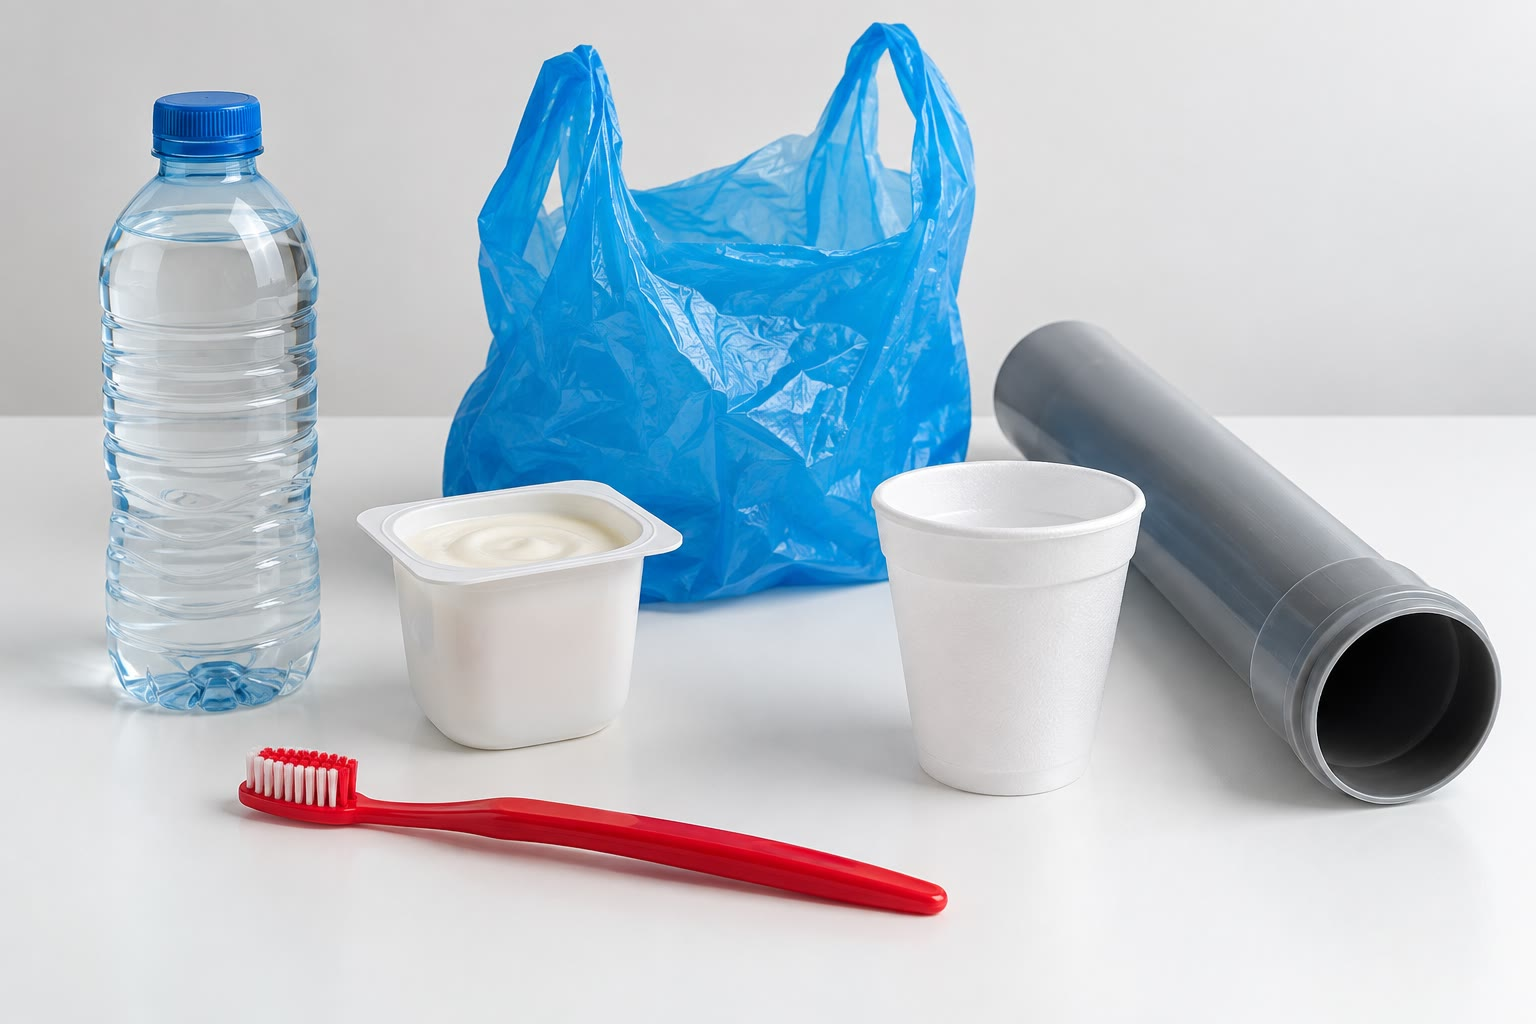
\includegraphics[width=0.55\linewidth]{images/book1/ai/g8-plastic-objects.jpg}

{\small Everyday \omterm{def:g8:plastics:plastic}{plastic} objects: a bottle, a pot, a bag, a pipe, a cup, a
toothbrush.}
\end{omfigure}

\section{Natural, artificial and synthetic materials}

\begin{definition}[Artificial and synthetic materials]\label{def:g8:plastics:artificial}
Among \omterm{def:g5:raw-materials-and-recycling:natural-material}{manufactured materials}, an \emph{artificial
material}\index{artificial material} is made by chemically transforming
a \omterm{def:g5:raw-materials-and-recycling:natural-material}{natural material}: paper and viscose (a fabric) from the cellulose of
wood. A \emph{synthetic material}\index{synthetic material} is made from
substances built by chemists, most often from crude oil, and has no
natural counterpart: nylon, polyester, the \omterm{def:g8:plastics:plastic}{plastics}.
\end{definition}

\begin{omfigure}
\begin{tikzpicture}[font=\small, level distance=1.5cm,
    box/.style={draw=omDef, fill=omDef!6, rounded corners=2pt, align=center,
      inner sep=4pt, text width=3.3cm},
    level 1/.style={sibling distance=6.4cm},
    level 2/.style={sibling distance=3.8cm},
    edge from parent/.style={draw, thick, omDef, ->}]
  \node[box] {materials}
    child {node[box] {natural\\ \footnotesize cotton, wool, wood}}
    child {node[box] {manufactured}
      child {node[box] {artificial\\ \footnotesize paper, viscose}}
      child {node[box, draw=omProp, fill=omProp!6] {synthetic\\ \footnotesize nylon,
        polyester, plastics}}};
\end{tikzpicture}

{\small Natural, artificial and \omterm{def:g8:plastics:artificial}{synthetic materials}.}
\end{omfigure}

\section{What plastics are}

\begin{definition}[Plastic]\label{def:g8:plastics:plastic}
A \emph{plastic}\index{plastic} is a \omterm{def:g8:plastics:artificial}{synthetic material} made of very
long \omterm{def:g7:atoms-and-molecules:molecule}{molecules}, which can be shaped by moulding --- most often while it
is hot and soft --- and keeps its shape when cool. Most plastics are made
from crude oil or natural gas.
\end{definition}

\begin{remark}[Very long molecules]\label{rem:g8:plastics:long}
A water \omterm{def:g7:atoms-and-molecules:molecule}{molecule} holds three \omterm{def:g7:atoms-and-molecules:atom}{atoms}; a \omterm{def:g7:atoms-and-molecules:molecule}{molecule} of a \omterm{def:g8:plastics:plastic}{plastic} can hold
tens of thousands, joined in a long chain, like a necklace of identical
beads. How such chains are built is the subject of a chapter at the end
of this book.
\end{remark}

\begin{omfigure}
\begin{tikzpicture}[font=\small]
  \foreach \k in {0,...,17} {
    \pgfmathsetmacro\x{0.62*\k}
    \pgfmathsetmacro\y{0.35*sin(40*\k)}
    \shade[ball color=omDef!50] (\x,\y) circle (0.22);
  }
  \node[anchor=west] at (11.2,0) {\dots};
  \node[anchor=north, align=center] at (5.3,-0.6) {a chain of thousands of identical units};
\end{tikzpicture}

{\small A picture, not a model: the \omterm{def:g7:atoms-and-molecules:molecule}{molecule} of a \omterm{def:g8:plastics:plastic}{plastic} is a very long
chain of identical units.}
\end{omfigure}

\begin{history}[Bakelite, 1907]
The first fully synthetic \omterm{def:g8:plastics:plastic}{plastic} was made by the chemist Leo Baekeland
in 1907, from phenol, obtained from coal tar, and formaldehyde. Bakelite, hard,
dark and heat-resistant, became the material of telephones, radios and
electric switches. Nylon followed in the 1930s, then the \omterm{def:g8:plastics:plastic}{plastics} of
bottles and bags after the Second World War.
\end{history}

\begin{omfigure}
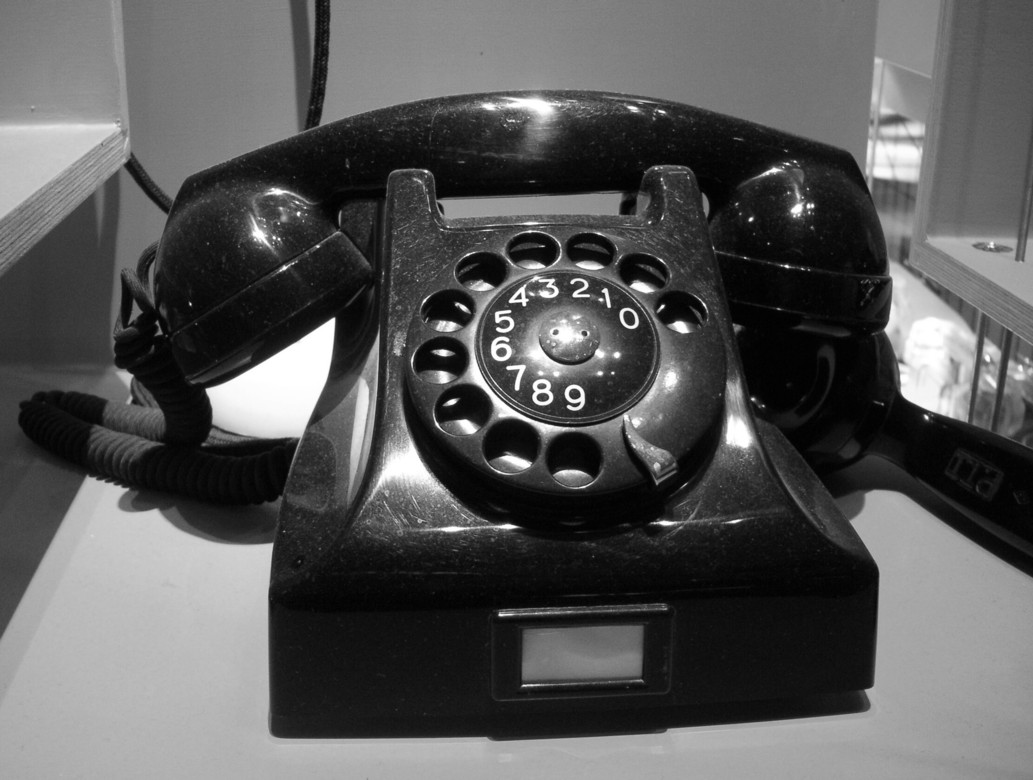
\includegraphics[width=0.42\linewidth]{images/book1/bakelite-telephone.jpg}

{\small A Bakelite telephone of 1947. Photo: Holger Ellgaard,
CC BY-SA 3.0.}
\end{omfigure}

\section{The main plastics and their codes}

\begin{definition}[Resin identification code]\label{def:g8:plastics:code}
The \emph{resin identification code}\index{resin identification code}
is a number from 1 to 7, printed inside a triangle of arrows on a
\omterm{def:g8:plastics:plastic}{plastic} object, that names the \omterm{def:g8:plastics:plastic}{plastic} it is made of, so that it can be
sorted for \omterm{def:g5:raw-materials-and-recycling:recycling}{recycling}. The triangle does not mean that the object will
be recycled.
\end{definition}

\begin{proposition}[Seven codes]\label{prop:g8:plastics:codes}
The codes, with the commonest uses of each \omterm{def:g8:plastics:plastic}{plastic}:
\begin{center}
\small
\begin{tabular}{cll}
\hline
code & \omterm{def:g8:plastics:plastic}{plastic} & typical objects \\
\hline
1 & PET, polyethylene terephthalate & water and soda bottles, fleece fibres \\
2 & HDPE, high-density polyethylene & milk and shampoo bottles, caps \\
3 & PVC, polyvinyl chloride & pipes, window frames, cables \\
4 & LDPE, low-density polyethylene & bags, films \\
5 & PP, polypropylene & yogurt pots, bottle caps, car bumpers \\
6 & PS, polystyrene & foam cups and trays, CD cases \\
7 & other \omterm{def:g8:plastics:plastic}{plastics} & \omterm{def:g6:pure-substances-and-mixtures:mixture}{mixtures}, multilayer packaging \\
\hline
\end{tabular}
\end{center}
\end{proposition}

\begin{omfigure}
\begin{tikzpicture}[font=\small]
  \foreach \n/\lab in {1/PET, 2/HDPE, 3/PVC, 4/LDPE, 5/PP, 6/PS, 7/OTHER} {
    \begin{scope}[xshift=(\n-1)*2.1cm]
      \foreach \a in {90,210,330} {
        \pgfmathsetmacro\b{\a+120}
        \draw[omDef, line width=1.1pt, ->, >={Stealth[length=4pt]}]
          ($(\a:0.75)!0.14!(\b:0.75)$) -- ($(\a:0.75)!0.86!(\b:0.75)$);
      }
      \node[font=\bfseries] at (0,-0.05) {\n};
      \node[anchor=north, font=\footnotesize] at (0,-0.8) {\lab};
    \end{scope}
  }
\end{tikzpicture}

{\small The seven \omterm{def:g8:plastics:code}{resin identification codes}, each with the short name of
its \omterm{def:g8:plastics:plastic}{plastic}.}
\end{omfigure}

\section{Thermoplastics and thermosets}

\begin{definition}[Thermoplastic and thermoset]\label{def:g8:plastics:thermoplastic}
A \emph{thermoplastic}\index{thermoplastic} softens each time it is
heated and hardens again when it cools: it can be melted and moulded
again and again (PET, polyethylene, PVC, polypropylene, polystyrene). A
\emph{thermoset}\index{thermoset} sets for good when it is first heated
and moulded: heated again, it does not soften but chars (Bakelite, the
resins of glues and of boat hulls).
\end{definition}

\begin{remark}[Which can be recycled]\label{rem:g8:plastics:which}
\omterm{def:g8:plastics:thermoplastic}{Thermoplastics} can be melted and remoulded: they are the \omterm{def:g8:plastics:plastic}{plastics} that
are recycled into new objects. \omterm{def:g8:plastics:thermoplastic}{Thermosets} cannot be melted again.
\end{remark}

\section{Plastics in the environment}

\begin{proposition}[Plastics last]\label{prop:g8:plastics:last}
% ledger: plastics:use-2019, plastics:waste-2019, plastics:recycled-share-2019
The world used about 460 million tonnes of \omterm{def:g8:plastics:plastic}{plastics} in 2019 and threw
away about 353 million tonnes of \omterm{def:g8:plastics:plastic}{plastic} waste; recycled \omterm{def:g8:plastics:plastic}{plastic} made up
only about \qty{6}{\percent} of the \omterm{def:g8:plastics:plastic}{plastic} used. \omterm{def:g8:plastics:plastic}{Plastics} do not rot:
in nature they break into smaller and smaller pieces, the microplastics,
which are found in rivers, oceans, soils and the bodies of animals.
\end{proposition}

\begin{omfigure}
\begin{minipage}[t]{0.48\linewidth}\centering
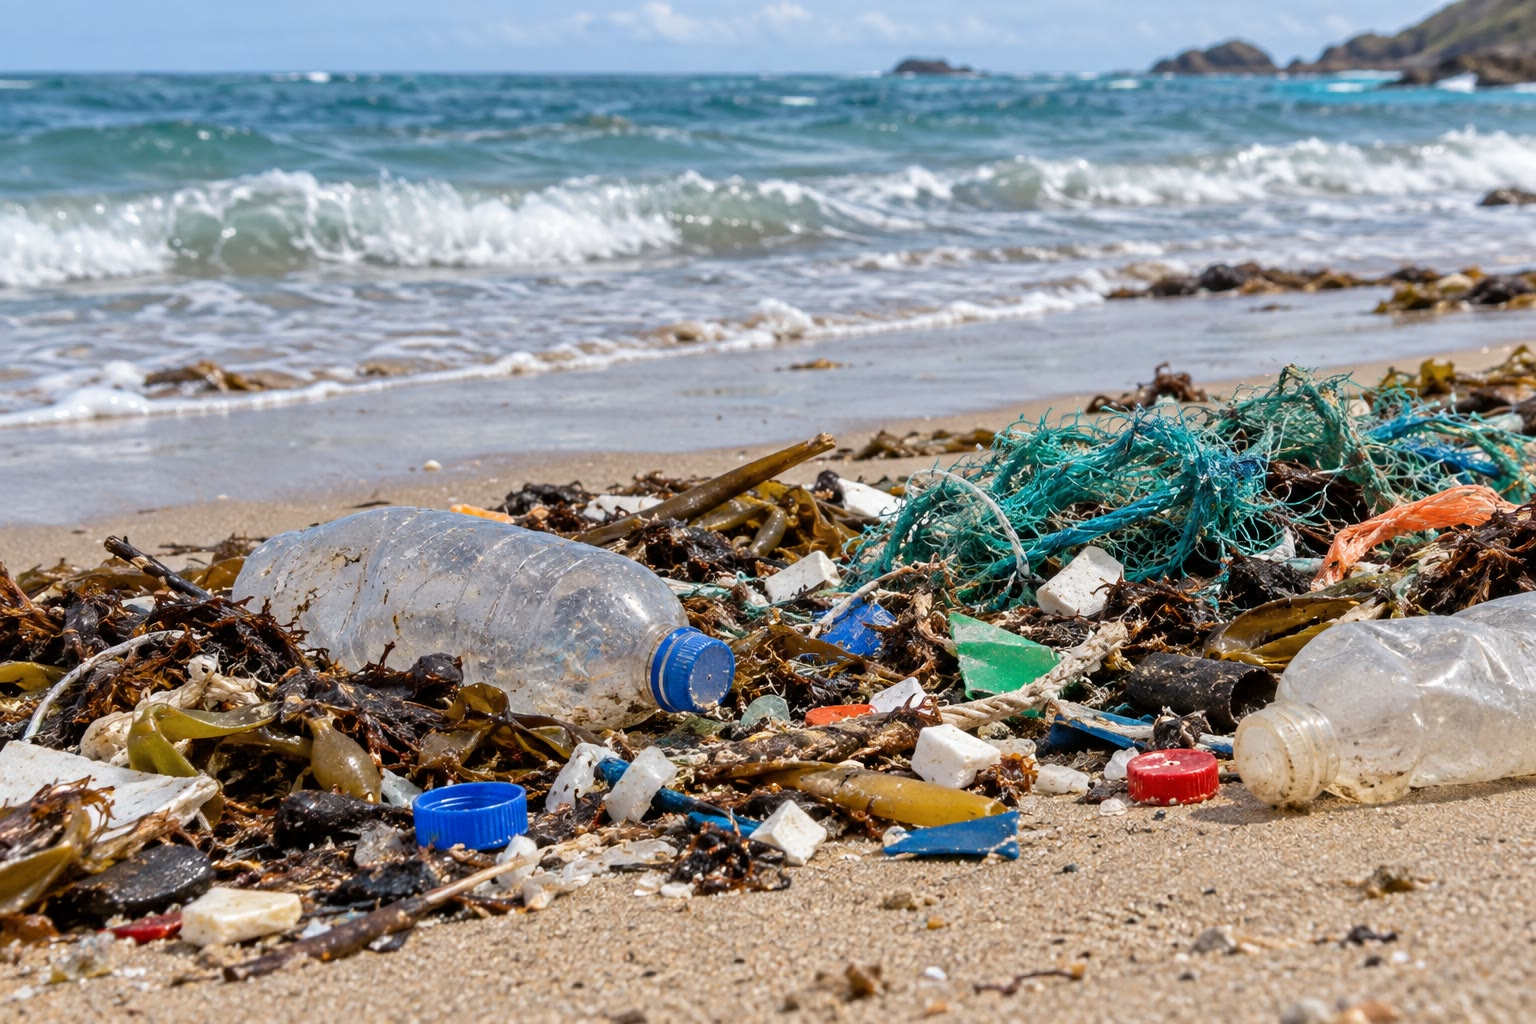
\includegraphics[width=\linewidth,height=4.6cm,keepaspectratio]{images/book1/ai/g8-beach-litter.jpg}

{\small \omterm{def:g8:plastics:plastic}{Plastic} litter washed up on a beach.}
\end{minipage}\hfill
\begin{minipage}[t]{0.48\linewidth}\centering
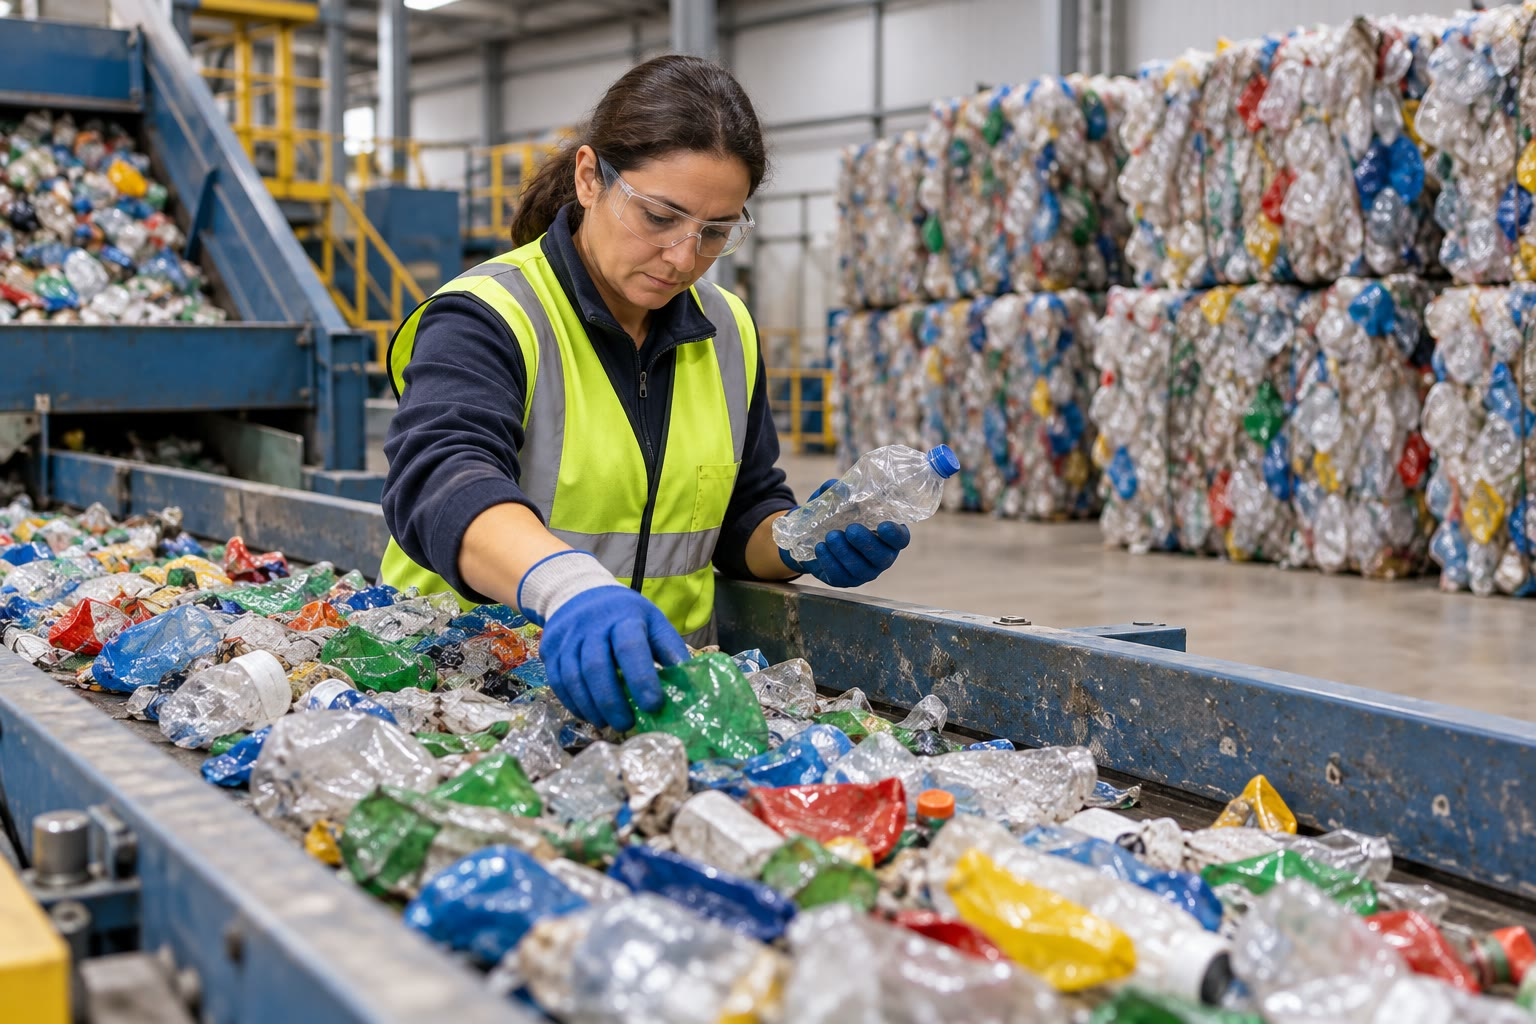
\includegraphics[width=\linewidth,height=4.6cm,keepaspectratio]{images/book1/ai/g8-sorting-line.jpg}

{\small A sorting line in a \omterm{def:g8:plastics:plastic}{plastics} \omterm{def:g5:raw-materials-and-recycling:recycling}{recycling} plant.}
\end{minipage}
\end{omfigure}

\begin{remark}[Burning plastics]\label{rem:g8:plastics:burning}
\omterm{def:g8:plastics:plastic}{Plastics} burn, and they make carbon dioxide when they burn completely.
But burnt in a garden fire they burn incompletely and release soot,
carbon monoxide and other harmful substances; PVC, which contains
chlorine, gives off hydrogen chloride, a corrosive gas. \omterm{def:g8:plastics:plastic}{Plastic} waste is
burnt only in incinerators built to clean their fumes.
\end{remark}

\section{Exercises}

\begin{exercise}[$\star$]\label{exo:g8:plastics:1}
Natural, artificial or synthetic? Cotton, nylon, paper, wool,
polystyrene, viscose.
\end{exercise}

\begin{exercise}[$\star$]\label{exo:g8:plastics:2}
From which \omterm{def:g5:raw-materials-and-recycling:raw-material}{raw material} are most \omterm{def:g8:plastics:plastic}{plastics} made?
\end{exercise}

\begin{exercise}[$\star$]\label{exo:g8:plastics:3}
Which \omterm{def:g8:plastics:plastic}{plastic} has the code 1? Give one object made of it.
\end{exercise}

\begin{exercise}[$\star$]\label{exo:g8:plastics:4}
What is the difference between a \omterm{def:g8:plastics:thermoplastic}{thermoplastic} and a \omterm{def:g8:plastics:thermoplastic}{thermoset}?
\end{exercise}

\begin{exercise}[$\star\star$]\label{exo:g8:plastics:5}
A yogurt pot carries the code 5. Name its \omterm{def:g8:plastics:plastic}{plastic}, and say whether it
could in principle be melted and remoulded.
\end{exercise}

\begin{exercise}[$\star\star$]\label{exo:g8:plastics:6}
Why does a triangle of arrows on an object not mean that the object will
be recycled?
\end{exercise}

\begin{exercise}[$\star\star$]\label{exo:g8:plastics:7}
Why is the handle of a frying pan often made of a \omterm{def:g8:plastics:thermoplastic}{thermoset} rather than a
\omterm{def:g8:plastics:thermoplastic}{thermoplastic}?
\end{exercise}

\begin{exercise}[$\star\star$]\label{exo:g8:plastics:8}
Using the figures of this chapter for 2019, what percentage of the
\omterm{def:g8:plastics:plastic}{plastic} used became waste that year? Round to the nearest whole number.
\end{exercise}

\begin{exercise}[$\star\star$]\label{exo:g8:plastics:9}
Why must PVC never be burnt in a garden fire?
\end{exercise}

\begin{exercise}[$\star\star$]\label{exo:g8:plastics:10}
A school uses 300 bottles of \qty{25}{g} each per week, during 36 weeks
of the year. What mass of \omterm{def:g8:plastics:plastic}{plastic} is that in a year?
\end{exercise}

\begin{exercise}[$\star\star\star$]\label{exo:g8:plastics:11}
Polyethylene is made of carbon and hydrogen only. Write the products of
its \omterm{def:g8:combustion-and-fuels:complete}{complete combustion}. Explain why \omterm{def:g4:what-a-fire-needs:burning}{burning} it adds carbon dioxide to
the \omterm{def:g4:air-a-mixture-of-gases:air}{air} like a \omterm{def:g8:combustion-and-fuels:fossil}{fossil fuel}.
\end{exercise}

\begin{exercise}[$\star\star\star$]\label{exo:g8:plastics:12}
Explain how a \omterm{def:g8:plastics:plastic}{plastic} bottle lost at sea can end up, years later, as
microplastics inside a fish.
\end{exercise}

\section{Problem: The Sorting Line}

\begin{problem}[{Weekend problem --- a tonne of used bottles, their
codes, and the clean plastic flakes that come out of the plant}]
\label{pb:g8:plastics:1}
A \omterm{def:g5:raw-materials-and-recycling:recycling}{recycling} plant receives bales of used drink bottles. A typical bale
of \qty{1}{t} (\qty{1000}{kg}) holds, by mass: \qty{80}{\percent} of
bottle bodies in PET, \qty{12}{\percent} of caps (HDPE and PP),
\qty{5}{\percent} of labels (PP film) and \qty{3}{\percent} of dirt and
leftover liquid. Machines separate the caps and labels from the bodies,
the PET is ground into flakes, and the flakes are washed; the washing
loses \qty{2.5}{\percent} of the PET. The clean flakes are melted and
spun into the fibres of fleece jackets.

\medskip
\noindent\textbf{Part I --- The \omterm{def:g8:plastics:plastic}{plastics}.}
\begin{enumerate}
  \item Which code is printed on the bottle bodies? On the caps?
  \item Are these \omterm{def:g8:plastics:plastic}{plastics} natural, artificial or synthetic?
  \item Can PET be melted and spun again? What kind of \omterm{def:g8:plastics:plastic}{plastic} does this
        make it?
  \item Why are the caps and labels separated from the bodies before the
        PET is melted?
\end{enumerate}

\medskip
\noindent\textbf{Part II --- The bale.}
\begin{enumerate}[resume]
  \item What mass of PET does a bale contain?
  \item What mass of caps? Of labels?
  \item What mass of the bale is not \omterm{def:g8:plastics:plastic}{plastic}?
  \item What percentage of the bale is \omterm{def:g8:plastics:plastic}{plastic}?
\end{enumerate}

\medskip
\noindent\textbf{Part III --- The flakes.}
\begin{enumerate}[resume]
  \item What mass of PET is lost in the washing?
  \item A fleece jacket needs \qty{0.39}{kg} of PET fibre. Why is it
        better to make it from flakes than from new PET?
  \item The plant could burn the caps and labels for heat instead of
        \omterm{def:g5:raw-materials-and-recycling:recycling}{recycling} them. Name the gas this would add to the \omterm{def:g4:air-a-mixture-of-gases:air}{air}.
  \item Compute the mass of clean PET flakes that one bale gives.
\end{enumerate}
\end{problem}
